\documentclass[compress]{beamer}
%\mode<presentation>
\usetheme{Madrid}
%\usetheme{Boadilla}
%\usetheme{AnnArbor}
%\usetheme{CambridgeUS}
\useoutertheme[footline=authortitle,subsection=false]{miniframes}
\usecolortheme{lily}
\setbeamerfont{normal text}{series=\mdseries}
\setbeamerfont{item}{series=\mdseries}
\setbeamerfont{itemize/enumerate body}{series=\mdseries}
\setbeamerfont{itemize/enumerate subbody}{series=\mdseries}
\usepackage{graphicx}
%\usepackage{caption}
%\usepackage{subcaption}
\usepackage{tikz}
\usepackage{pgfplots}
\usepackage{booktabs}
\newcommand{\mykeywords}{Casino effects on Population and Family Formation}

%\usepackage{enumitem}% http://ctan.org/pkg/enumitem
\setbeamercolor{section in toc}{fg=dark_blue}
\setbeamercolor{itemize item}{fg=dark_blue}
\usepackage{color}
\usepackage{subcaption}
\usepackage{hyperref}
\usepackage{pdfpages}
\usepackage{appendixnumberbeamer}
\usepackage{babel,blindtext}
%\usepackage{beamerthemesplit} % Activate for custom appearance
%%%%%%%%%%%%%%%%%%%%%%%%%%%%%%%%%%%%%%%%%%%%%%%%%%
\definecolor{purple}{RGB}{128,100,162}
\definecolor{dk_purple}{RGB}{96,75,120}
\definecolor{maroon}{RGB}{149,55,53}
\definecolor{lt_maroon}{RGB}{175,101,65}
\definecolor{mute_blue}{RGB}{55,96,146}
\definecolor{mute_green}{RGB}{79,130,40}
\definecolor{dark_blue}{RGB}{32,64,97}
\definecolor{lt_green}{RGB}{195, 214, 155}
\definecolor{grey}{RGB}{125, 125, 125}
\definecolor{green}{RGB}{0, 182, 0}
\definecolor{blue}{RGB}{0, 0, 255}
\definecolor{teal}{RGB}{0, 105,128}
%%%%%%%%%%%%%%%%%%%%%%%%%%%%%%%%%%%%%%%%%%%%%%
\setbeamercolor{title}{fg=dark_blue}
\setbeamercolor{frametitle}{fg=dark_blue}
%\setbeamertemplate{footline}{}
\setbeamertemplate{footline}{%
  \leavevmode%
  \hbox{%
    \begin{beamercolorbox}[wd=.73\paperwidth,ht=2.5ex,dp=1ex,left]{title in head/foot}%
      \usebeamerfont{title in head/foot}%
      \mykeywords \hspace{1em}--\hspace{1em} \insertsubsectionhead
    \end{beamercolorbox}%
    \begin{beamercolorbox}[wd=.33\paperwidth,ht=2.5ex,dp=1ex,right]{date in head/foot}%
      \usebeamerfont{date in head/foot}%
      \insertshortdate{}\hspace*{2ex}%
      \insertframenumber{} / \inserttotalframenumber\hspace*{2ex}%
    \end{beamercolorbox}%
  }%
  \vskip0pt%
}
\setbeamerfont{footnote}{series=\mdseries}
\usepackage{caption}
\captionsetup[figure]{labelformat=empty}% redefines the caption setup of the figures environment in the beamer class.
\usefonttheme{professionalfonts}
\usepackage[style=authoryear, backend=bibtex]{biblatex}
\addbibresource{casino.bib} 
\renewcommand*{\nameyeardelim}{\addcomma\addspace}
\let\oldparencite\parencite
\renewcommand{\parencite}[1]{{\mdseries\oldparencite{#1}}}

\title{The Destruction of Social Capital and Family Flight: Evidence from Casino Openings}
\subtitle{South Dakota Land and Lending Conference Presentation}
\author{
	Malcolm Kass \& 
	John Soriano \\
	\vspace{0.5cm}
    {\it University of Dallas} \\
	\href{mailto:mkass@udallas.edu}{mkass@udallas.edu} \\
    \href{mailto:jsoriano@udallas.edu}{jsoriano@udallas.edu} }
    
\date{\today}


\begin{document}
	
	\begin{frame}
		\titlepage
	\end{frame}


\section{Introduction}
\begin{frame} \frametitle{Effect of new casino development on Population and Family Dynamics}
	\begin{itemize}
		\item Possibility of Resort style Casino Gambling in Texas: \href{https://www.dallasnews.com/news/politics/2025/06/30/what-to-know-about-las-vegas-sands-the-casino-giant-betting-big-on-north-texas/}{\color{blue}Proposed Sands Casino in Irving, Texas}  
        \item Proposed Irving location close to University of Dallas \begin{itemize}
            \item Irving, TX: Pop: 260k, Inner-ring suburb
            \item Lower Median Income for DFW (79k), but similar to the rest of Texas/US
            \item Highly Diverse: Demographics and Income
        \end{itemize}
        \item Why Irving?
        \begin{itemize}
        \item First mover, but not a current destination area. 
        \item Location is a self-contained, large empty plot: Little to no economic spillovers. Akin to a \textit{walled medieval European city }
        \item[] \href{https://maps.app.goo.gl/6p2Zy9oHBkHnfjDT7}%
{\beamergotobutton{Open Interactive Map}}
        \end{itemize}
    \end{itemize}
\end{frame}




\begin{frame} \frametitle{Related Previous Work}
	\begin{itemize}
		\item Increased Crime: Casinos caused increases in aggravated assault, rape, robbery, larceny, burglary, auto theft \parencite{grinols2006casinos}
        \begin{itemize}
        \item All 3,165 U.S. counties from 1977 to 1996
        \item Initially small, growing significantly after 3-5 years
        \item Magnitude: 8.6\% of property crime and 12.6\% of violent crime in casino counties attributable to casinos 
        \end{itemize}
        \item Increases in Economic Outcomes
        \begin{itemize}
            \item Retail Property values \parencite{wiley2011casino} 
            \item Increases in Hospitality Industry employment \parencite{humphreys2013new}
        \end{itemize}
        \item Unique for this project: destination areas not included \& no preexisting casino presence
    \end{itemize}
\end{frame}

\begin{frame} \frametitle{Research Contribution and Preliminary Results}
	\begin{itemize}
		\item Novel work on how a new casino entrant affects marriage, fertility, and population composition, setting akin to Sands' entry into Irving
        \item Unclear direction: Crime increases (-) vs. Employment gains (+)
        \item []
        \item [] Initial Results
        \item Casino $\rightarrow$ County level population drops, long-time resident families moving out
        \item Casino $\rightarrow$ 1.28 percentage point decline in fertility rates for women
    \end{itemize}
\end{frame}


\section{Data and Methods}
\begin{frame} \frametitle{Explanatory variable of interest: 2003-2023 US county-level casino openings}
	\begin{itemize}
    \item Students in UD's 2025 Advanced Econometrics created a database of new casino openings by county and adjacent counties from 2003 to 2023 (to match timeframe of ATUS data)
    \item Denoted counties with preexisting casinos before 2003. 
    \item Research Design aligned with UD's Sands situation. 
\item []
        \item [] \textbf{Treatment:} New casino counties. Only includes new casino counties in the data time frame, no previous casinos or additional casinos. (66 total) 
        \item [] \textbf{Control:} No Casino or casino adjacent counties to prevent spillovers clouding effects
	\end{itemize}
\end{frame}

\begin{frame} \frametitle{Explanatory variable of interest: 2003-2023 US county-level casino openings}
\begin{figure}[H]
\centering
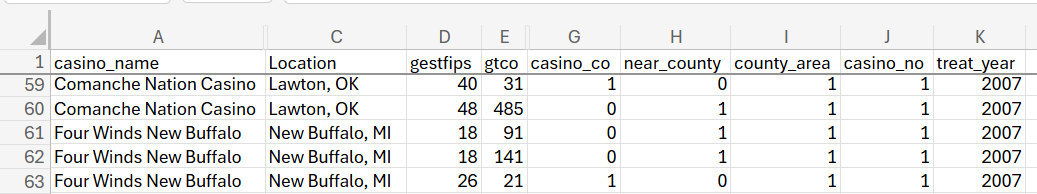
\includegraphics[width=12cm]{shot_casino.png}
\end{figure}
\end{frame}

\begin{frame} \frametitle{Dependent Variables: population and family formation measures}
	\begin{itemize}
    \item ACS micro data from 2000-2023 
	\item Adult and Child Population data: 
    \begin{itemize}
        \item Total, Child Rearing (18 to 40), Children ($\le$ 17), School age (5-17)
    \end{itemize}
    \item Family and fertility data: 
    \begin{itemize}
        \item marital status (base: not married currently)
        \item has children
        \item number of children
    \end{itemize}
    		\item Notable aggregate differences between treatment casino counties vs. control counties
        \begin{itemize}
            \item 31.3\% vs 37.9\% marriage rates
            \item 0.70 vs 0.82 children per person
            \item 28.7\% vs 17.8\% Hispanic representation
        \end{itemize}
	\end{itemize}
\end{frame}

\begin{frame} \frametitle{Methods}
		\begin{itemize}
	\item Staggered Difference and Differences estimated with two-way fixed effects (FE) specification:
    \item [] \begin{equation}
Y_{ct} = \alpha + \beta \cdot \text{Post}_{ct} + \mathbf{X}_{ct}'\gamma + \mu_c + \lambda_t + \varepsilon_{ct}
\end{equation}
    \begin{itemize}
        \item $Y_{ct}$ is the DV in county $c$ and year $t$ 
        \item $\text{Post}_{ct}$ is an indicator equal to one if county $c$ has an operating casino in year $t$
        \item $\mathbf{X}_{ct}$ includes demographic controls 
        \item $\mu_c$ and $\lambda_t$ are county and year fixed effects
        \item Standard errors clustered at the county level
        \item Weighted by overall population (low population county averages do not hold the same weight as densely populated counties) 
	\end{itemize}
\end{itemize}
\end{frame}

\begin{frame} \frametitle{Staggered Difference and Differences (DiD):}
	\begin{itemize}
    \item Causal technique to estimate treatment effects (new casino)
     \item In many applications, we want to estimate the effect of a policy or economic change
    \item However, the policy assignment is not necessarily uncorrelated with group characteristics
    \begin{itemize}
        \item A new casino may be located specifically in treated areas with declining population and family formation
        \item DiD uses, as a control, areas that were never treated 
    \end{itemize}
    \item The treatment effect (effect of the casino) is the difference in the DV of the treated areas minus the difference in the DV of the control areas.
    \item Fixed Effects estimation accounts for county and time-specific effects that may confound results 
\end{itemize}
\end{frame}

\section{Results, Mechanisms, Conclusion}
\begin{frame} \frametitle{Results for log population by age group}
\begin{figure}[H]
\centering
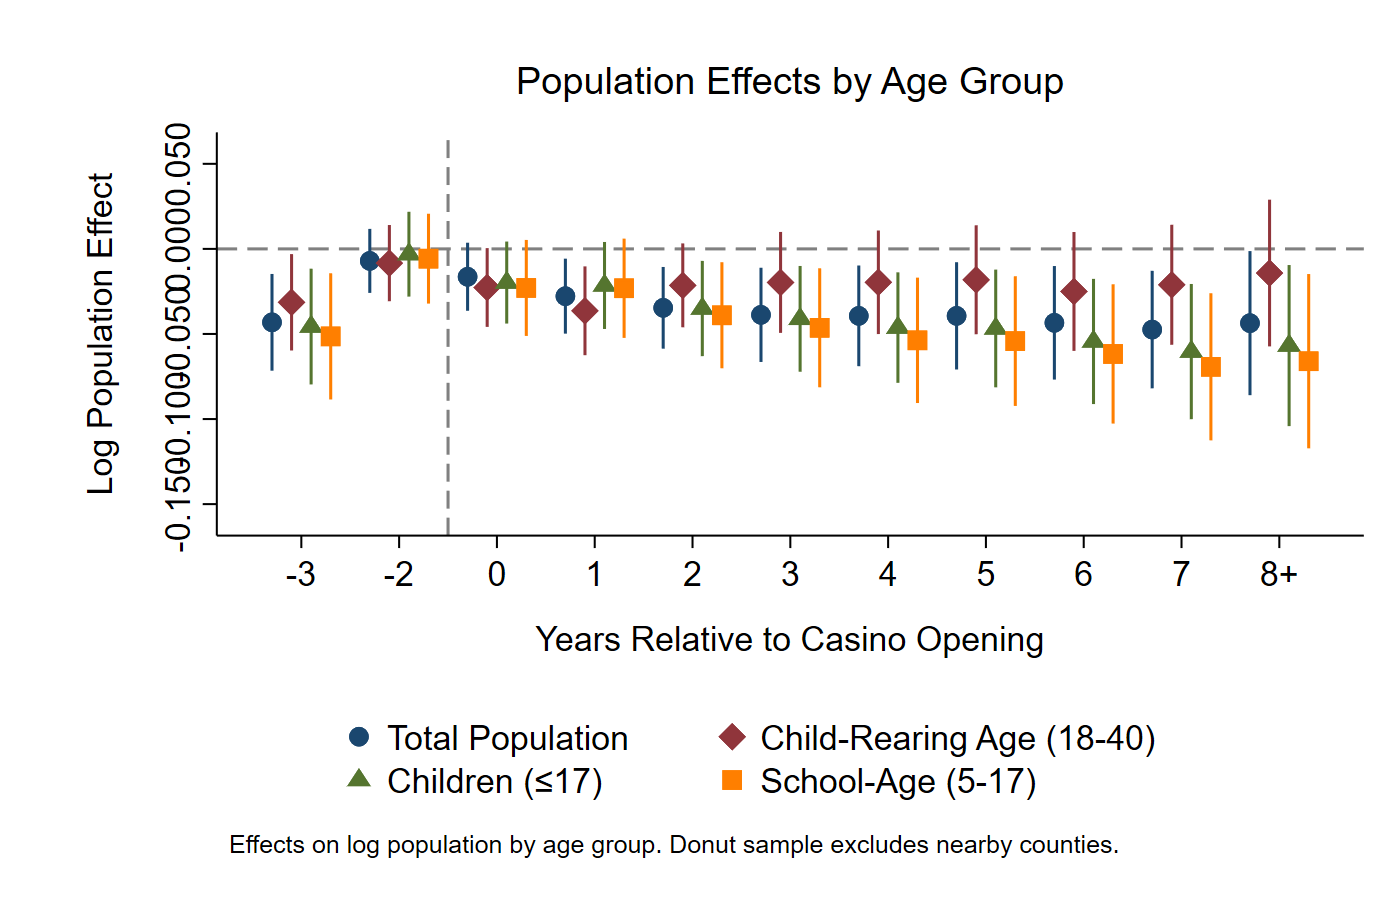
\includegraphics[width=10cm]{figure1_population_effects.png}
\end{figure}
Stronger effects on children relative to adults suggest family formation vs. general population decline \\
\end{frame}

\begin{frame} \frametitle{Diff and Diff results on Fertility}
\begin{table}[htbp]\centering
\def\sym#1{\ifmmode^{#1}\else\(^{#1}\)\fi}
\scriptsize
\begin{tabular}{l*{6}{c}}
\hline\hline
            &\multicolumn{3}{c}{Women}                                        &\multicolumn{3}{c}{Men}                                          \\\cmidrule(lr){2-4}\cmidrule(lr){5-7}
            &\multicolumn{1}{c}{(1)}&\multicolumn{1}{c}{(2)}&\multicolumn{1}{c}{(3)}&\multicolumn{1}{c}{(4)}&\multicolumn{1}{c}{(5)}&\multicolumn{1}{c}{(6)}\\
            &\multicolumn{1}{c}{Marriage}&\multicolumn{1}{c}{Child}&\multicolumn{1}{c}{Num Kids}&\multicolumn{1}{c}{Marriage}&\multicolumn{1}{c}{Child
            }&\multicolumn{1}{c}{Num Kids}\\
\hline
post\_treat&      0.0046         &     -0.0128\sym{***}&     -0.0551\sym{***}&      0.0048         &     -0.0045         &     -0.0262\sym{***}\\
            &    (0.0041)         &    (0.0043)         &    (0.0138)         &    (0.0032)         &    (0.0033)         &    (0.0089)         \\
\hline
Obser&   9,135,596         &   9,135,596         &   9,135,596         &   9,230,246         &   9,230,246         &   9,230,246         \\
R-squared   &       0.206         &       0.267         &       0.239         &       0.218         &       0.225         &       0.203         \\
\hline\hline
\multicolumn{7}{l}{\footnotesize Standard errors in parentheses}\\
\multicolumn{7}{l}{\footnotesize All regressions include county and year fixed effects, $age$ and $age^2$}\\
\multicolumn{7}{l}{\footnotesize \sym{*} \(p<0.10\), \sym{**} \(p<0.05\), \sym{***} \(p<0.01\)}\\
\end{tabular}
\end{table}
Larger fertility effects for women are consistent with greater control over reproductive decisions.  \\
\end{frame}

\begin{frame} \frametitle{Fertility}
\begin{figure}[H]
\centering
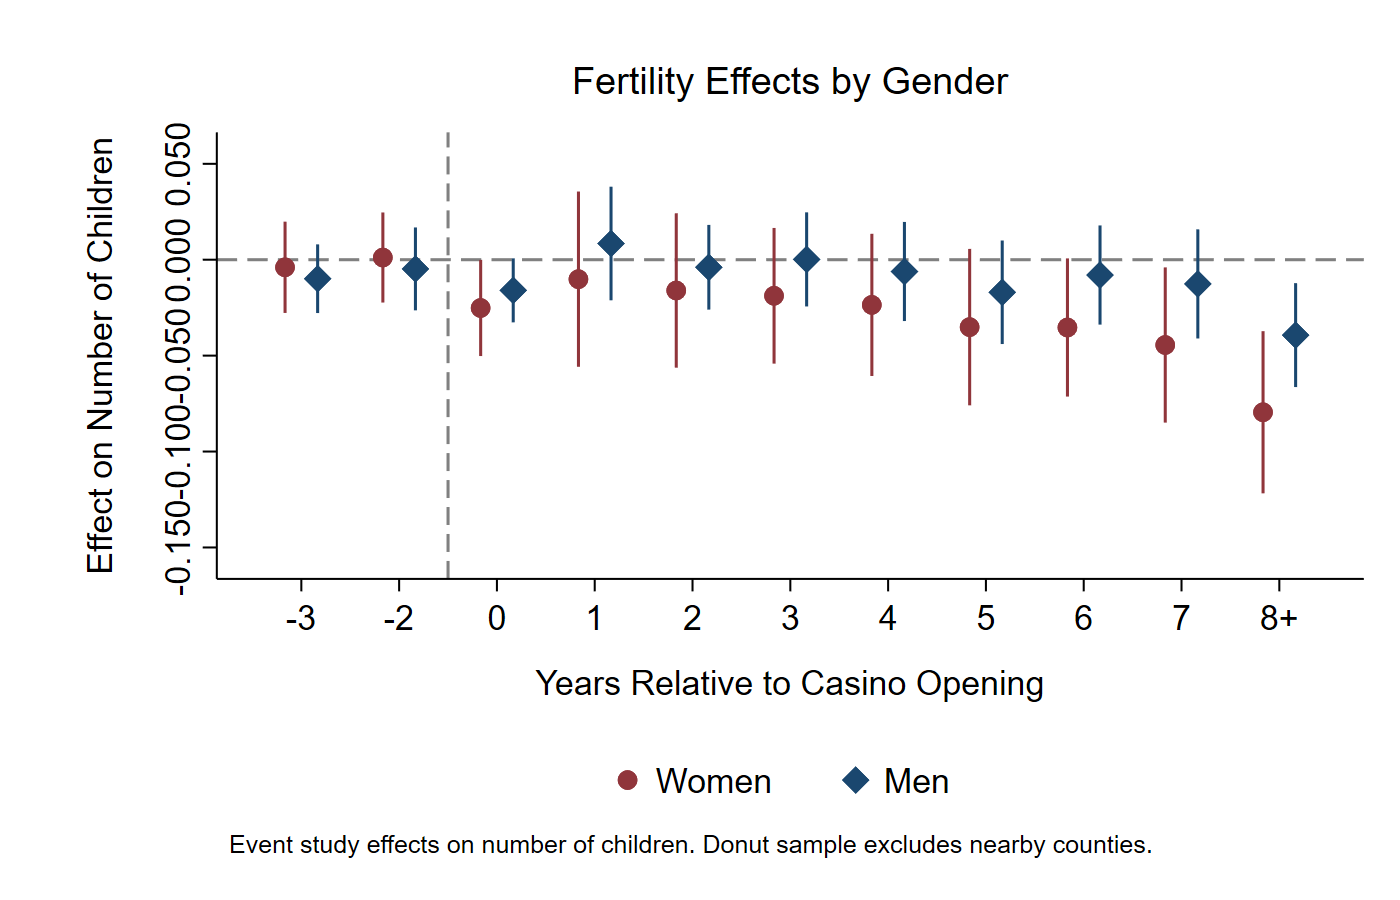
\includegraphics[width=10cm]{figure2_fertility_effects.png}
\end{figure}
Fertility effects emerge immediately after casino opening and persist throughout our observation window. \\
\end{frame}

\begin{frame} \frametitle{Fertility Mechanism}
\begin{figure}[H]
\centering
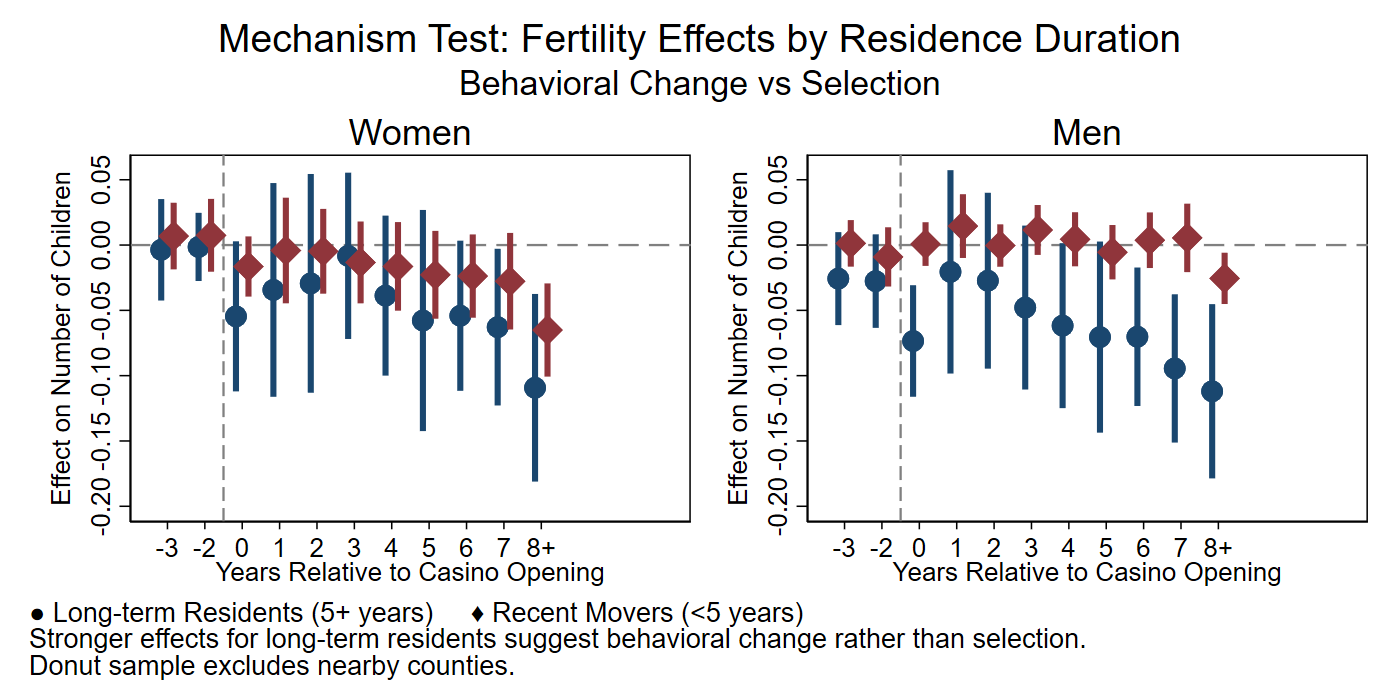
\includegraphics[width=10cm]{figure3_mechanism_test.png}
\end{figure}
Drop in fertility for long-term residents at casino opening. Suggests selective out-migration of family-oriented long-term residents rather than behavioral change.\\
\end{frame}

\begin{frame} \frametitle{Conclusion}
	\begin{itemize}
    \item Evidence that casinos systematically disrupt populations and family formation
    \item Family disruption operates via selective out-migration of family-oriented long-term residents, not necessarily behavior change. 
    \item The magnitude of these effects is substantial: fertility declines by 3-6\% and child populations fall by 5-6\%. These changes persist and intensify over our 8+ year observation window.
    \item Moving forward: It is unclear whether out-migration is due to the presence of the casino or the character makeup of transplants. Alter the form of our DV to inflows. 
	\end{itemize}
\end{frame}


\begin{frame} \frametitle{Thank you.}
\begin{figure}[H]
\centering
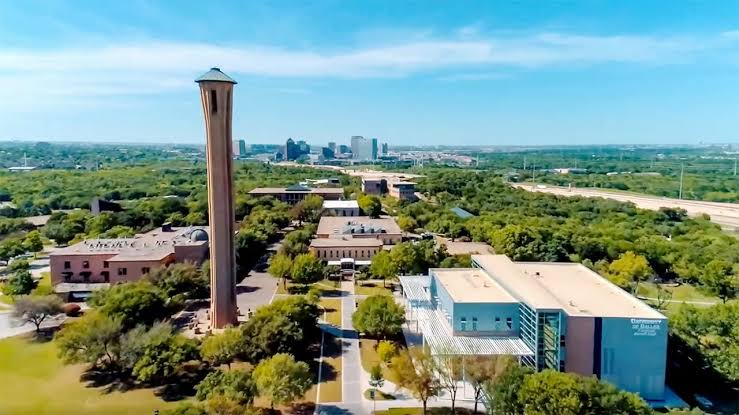
\includegraphics[width=12cm]{ud.png}
\end{figure}
\end{frame}

\appendix
\begin{frame}[noframenumbering,plain,label=hidden1]
Click to open the interactive map: 
\href{https://www.google.com/maps/embed?pb=!1m14!1m12!1m3!1d13617.557942782103!2d-96.90770995811222!3d32.844874030741465!2m3!1f0!2f0!3f0!3m2!1i1024!2i768!4f13.1!5e1!3m2!1sen!2sus!4v1759084871221!5m2!1sen!2sus}%
{\beamergotobutton{Open Interactive Map}}
\end{frame}

\begin{frame} \frametitle{School Pop \& Enrollment — Event-Study Summary}
\begin{table}[htbp]\centering
\scriptsize
\caption{Event-Study: School-Age Population \& Enrollment (Log DV)}
\begin{tabular}{lccc}
\hline\hline
Event Time & School-Age Pop & Total Enroll. & Public Enroll. \\
\hline
t-3   & -0.051*** & -0.049**  & -0.040**  \\
t-2   & -0.006    & -0.001    &  0.009    \\
t     & -0.023    & -0.019    & -0.023    \\
t+1   & -0.023    & -0.017    & -0.004    \\
t+2   & -0.039**  & -0.034**  & -0.020    \\
t+3   & -0.046*** & -0.042**  & -0.026    \\
t+4   & -0.054*** & -0.052*** & -0.028    \\
t+5   & -0.054*** & -0.052*** & -0.031    \\
t+6   & -0.062*** & -0.056*** & -0.028    \\
t+7   & -0.069*** & -0.064*** & -0.047**  \\
t+8+  & -0.066**  & -0.064**  & -0.038    \\
\hline\hline
\multicolumn{4}{l}{\footnotesize Stars indicate significance; SEs omitted for clarity.}\\
\end{tabular}
\end{table}

\end{frame}


\begin{frame} \frametitle{Religious Adherence}
\begin{table}[htbp]\centering
\scriptsize
\def\sym#1{\ifmmode^{#1}\else\(^{#1}\)\fi}
\caption{Spillover Effects: Casino vs Nearby Counties}
\begin{tabular}{l*{4}{c}}
\hline\hline
            &\multicolumn{1}{c}{(1)}&\multicolumn{1}{c}{(2)}&\multicolumn{1}{c}{(3)}&\multicolumn{1}{c}{(4)}\\
            &\multicolumn{1}{c}{Fertility (W)}&\multicolumn{1}{c}{Fertility (M)}&\multicolumn{1}{c}{Child Pop}&\multicolumn{1}{c}{Religious}\\
\hline
Casino County × Post&     -0.0433\sym{**} &     -0.0205\sym{**} &     -0.0253         &      9.8971         \\
            &    (0.0180)         &    (0.0086)         &    (0.0187)         &   (24.5977)         \\
[1em]
Nearby County × Post&     -0.0256         &     -0.0106         &     -0.0158         &    -42.1267         \\
            &    (0.0361)         &    (0.0272)         &    (0.0289)         &   (31.4860)         \\
\hline
Observations&    10381166         &    10476298         &       9,160         &       9,418         \\
R-squared   &       0.240         &       0.205         &       0.992         &       0.932         \\
\hline\hline
\multicolumn{5}{l}{\footnotesize Standard errors in parentheses}\\
\multicolumn{5}{l}{\footnotesize Tests for spillover effects to nearby counties. Justifies donut design.}\\
\multicolumn{5}{l}{\footnotesize \sym{*} \(p<0.10\), \sym{**} \(p<0.05\), \sym{***} \(p<0.01\)}\\
\end{tabular}
\end{table}
\end{frame}

\begin{frame} \frametitle{Spillover effects on nearby counties}
\begin{table}[htbp]\centering
\scriptsize
\def\sym#1{\ifmmode^{#1}\else\(^{#1}\)\fi}
\caption{Spillover Effects: Casino vs Nearby Counties}
\begin{tabular}{l*{4}{c}}
\hline\hline
            &\multicolumn{1}{c}{(1)}&\multicolumn{1}{c}{(2)}&\multicolumn{1}{c}{(3)}&\multicolumn{1}{c}{(4)}\\
            &\multicolumn{1}{c}{Fertility (W)}&\multicolumn{1}{c}{Fertility (M)}&\multicolumn{1}{c}{Child Pop}&\multicolumn{1}{c}{Religious}\\
\hline
Casino County × Post&     -0.0433\sym{**} &     -0.0205\sym{**} &     -0.0253         &      9.8971         \\
            &    (0.0180)         &    (0.0086)         &    (0.0187)         &   (24.5977)         \\
[1em]
Nearby County × Post&     -0.0256         &     -0.0106         &     -0.0158         &    -42.1267         \\
            &    (0.0361)         &    (0.0272)         &    (0.0289)         &   (31.4860)         \\
\hline
Observations&    10381166         &    10476298         &       9,160         &       9,418         \\
R-squared   &       0.240         &       0.205         &       0.992         &       0.932         \\
\hline\hline
\multicolumn{5}{l}{\footnotesize Standard errors in parentheses}\\
\multicolumn{5}{l}{\footnotesize Tests for spillover effects to nearby counties. Justifies donut design.}\\
\multicolumn{5}{l}{\footnotesize \sym{*} \(p<0.10\), \sym{**} \(p<0.05\), \sym{***} \(p<0.01\)}\\
\end{tabular}
\end{table}
Casino county fertility declines of 4.33\% for women and 2.05\% for men. Nearby county effects 2.56\% for women and 1.06\% for men, though not statistically significant.
\end{frame}

\end{document}

\begin{frame}{Event-Study Plot: School Pop \& Enrollment}
\centering
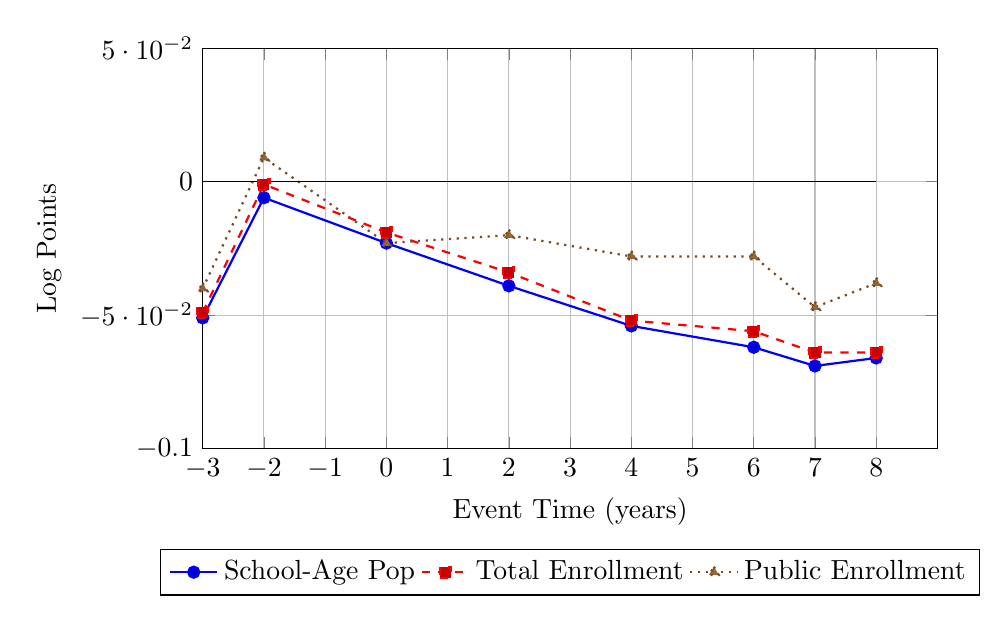
\begin{tikzpicture}
\begin{axis}[
    width=0.9\textwidth,
    height=0.55\textwidth,
    xlabel={Event Time (years)},
    ylabel={Log Points},
    xmin=-3, xmax=9,
    ymin=-0.10, ymax=0.05,
    xtick={-3,-2,-1,0,1,2,3,4,5,6,7,8},
    ytick={-0.10,-0.05,0,0.05},
    grid=major,
    legend style={at={(0.5,-0.25)},anchor=north,legend columns=-1},
    legend cell align=left
]

% Example line: School-Age Pop
\addplot+[mark=*, thick] coordinates {
    (-3,-0.051) (-2,-0.006) (0,-0.023) (2,-0.039) (4,-0.054) (6,-0.062) (7,-0.069) (8,-0.066)
};
\addlegendentry{School-Age Pop}

% Example line: Total Enrollment
\addplot+[mark=square*, thick, dashed] coordinates {
    (-3,-0.049) (-2,-0.001) (0,-0.019) (2,-0.034) (4,-0.052) (6,-0.056) (7,-0.064) (8,-0.064)
};
\addlegendentry{Total Enrollment}

% Example line: Public Enrollment
\addplot+[mark=triangle*, thick, dotted] coordinates {
    (-3,-0.040) (-2,0.009) (0,-0.023) (2,-0.020) (4,-0.028) (6,-0.028) (7,-0.047) (8,-0.038)
};
\addlegendentry{Public Enrollment}

% Horizontal zero line
\addplot[black, thin] coordinates {(-3,0) (8,0)};

\end{axis}
\end{tikzpicture}

\footnotesize 95\% CIs omitted for readability; full regression table in appendix.
\end{frame}

